\chapter{MCTゲートの分解手法}
本章では,既存のMCTゲートの\bout{分解手法\cite{abdessaied2016technology,baker2019decomposing,niemann2019t}}について説明する.
以降では,MCTゲートのコントロールビットの数を$c$とする.
\section{手法~1}
本節では,$c-2$個の値が不定の補助ビットを使用するMCTゲートの分解手法\cite{abdessaied2016technology}について説明する.
以降,本手法を手法~1と呼ぶ.
\bout{手法~1は,}
MCTゲートをToffoliゲートへ分解する手法\cite{barenco1995elementary}のT-depthを削減する手法である.
手法~1では,Toffoliゲートを位相のずれた$CCiZ, CCi\omega Z$ゲートに置換することで,T-depthを削減する.
\par
\mout{MCTゲートをToffoliゲートに分解した後,
これらのToffoliゲートを$CCiZ$ゲート,$CCi\omega Z$ゲートに置換する方法について説明する.
手法~1では,最初にToffolliゲートを$CCZ$ゲートとHゲートに置換する.
図~\ref{toffoli_transform}に示すように,ToffoliゲートはHゲートと$CCZ$ゲートに置換できる.
このため,図~\ref{barenco}中の,Toffoliゲートは図~\ref{toffoli_to_ccz}に示すように$CCZ$ゲートとHゲートに置換できる.}
\begin{figure}[tbp]
  \centering
  \begin{minipage}[b]{0.8\columnwidth}
    \centering
    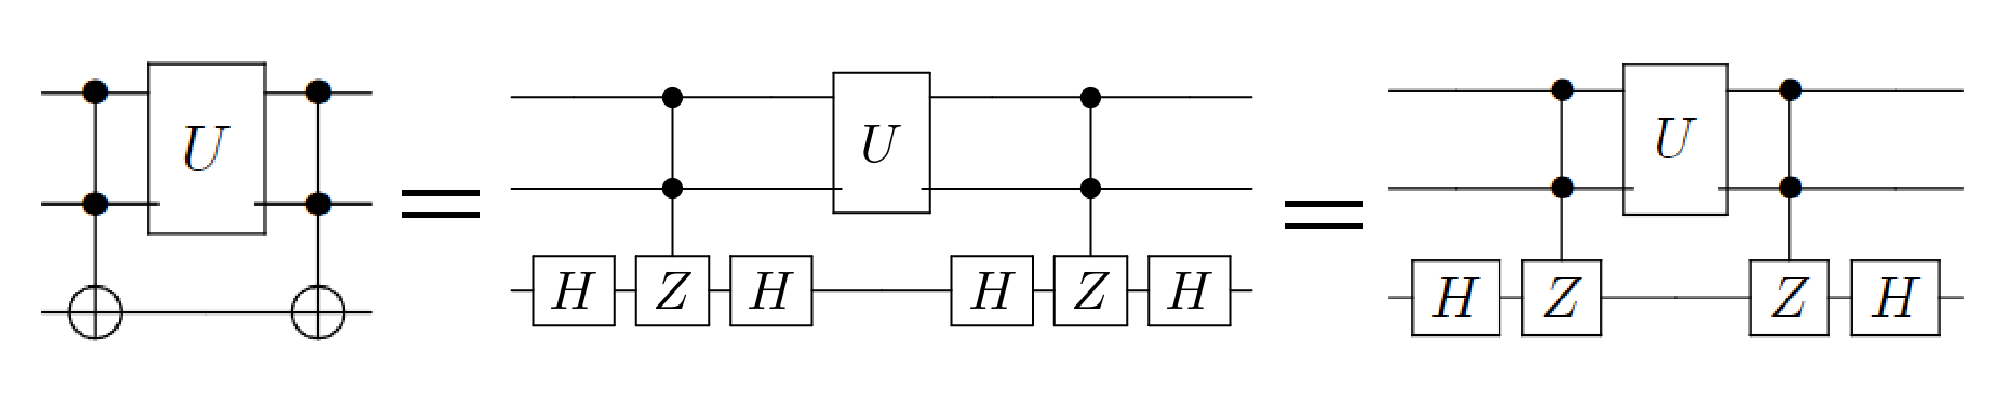
\includegraphics[width=0.9\columnwidth]{img/toffoli_transform.pdf}
    \caption{Toffoliゲートの$CCZ$ゲートへの置換}
    \label{toffoli_transform}    
  \end{minipage}
  \begin{minipage}[b]{0.4\columnwidth}
    \centering
    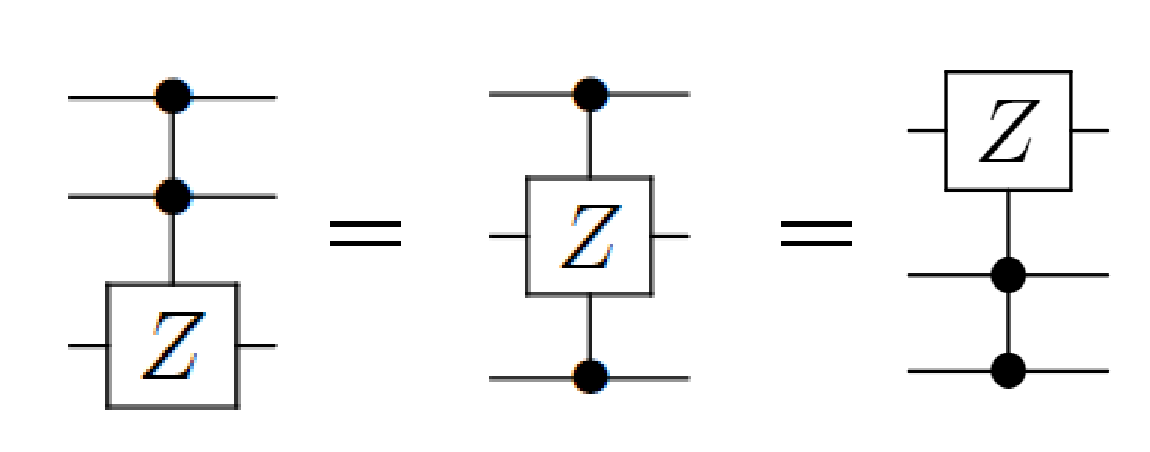
\includegraphics[width=0.9\columnwidth]{img/zgate_transform.pdf}
    \caption{$CCZ$ゲートの変形}
    \label{zgate_transform}    
  \end{minipage}
\end{figure}
\begin{figure}[tbp]
  \centering
  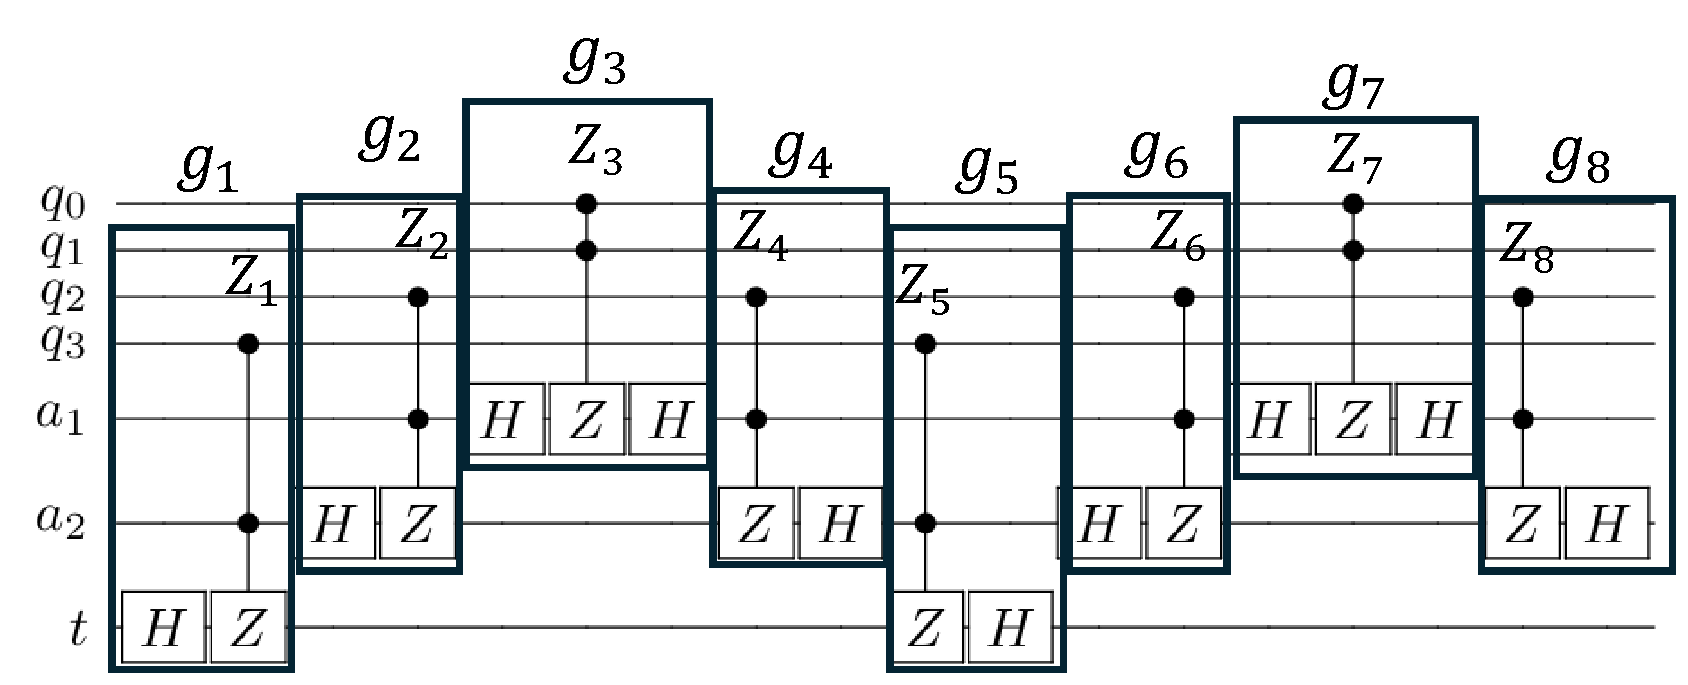
\includegraphics[width=13cm]{img/toffoli_to_ccz.pdf}
  \caption{図~\ref{barenco}のToffoliゲートを$CCZ$ゲートとHゲートに置換した例}
  \label{toffoli_to_ccz}
\end{figure} 
\par
\mout{次に,置換した$CCZ$ゲートを,$CCiZ$ゲートに置換する方法を説明する.
$CCZ$ゲートは,図~\ref{zgate_transform}に示すように,コントロールビットとターゲットビットを同一に見なすことができる.
また,図~\ref{zgate_to_iz}に示すように,$CCZ$ゲートは,
$CCiZ, CS$ゲートか,$CCiZ^{\dag}, CS^{\dag}$ゲートに置換できる.
このため,図~\ref{ccz_to_iz_cs}に示すように,図~\ref{toffoli_to_ccz}中の$CCZ$ゲートを$CCiZ, CS$ゲートと$CCiZ^{\dag}, CS^{\dag}$ゲートに置換できる.
図~\ref{ccz_to_iz_cs}では,図~\ref{toffoli_to_ccz}中の,
向かい合うゲート$\{Z_{1}. Z_{5}\}, \{Z_{2}, Z_{4}\}, \{Z_{3}, Z_{7}\},\{Z_{6}, Z_{8}\}$の組
をそれぞれ$CCiZ, CS$ゲート,$CCiZ^{\dag}, CS^{\dag}$ゲートの組に置換している.
これらの向かい合う$CCZ$ゲートを置換する際,
置換後の$CS, CS^{\dag}$ゲートの間で演算が生じない位置になるよう置換する.
例えば,$Z_{3}, Z_{7}$の組であれば,
置換後の$CS, CS^{\dag}$ゲート間で演算が生じないよう,
$CS, CS^{\dag}$ゲートのコントロールビットが$q_{0}$に,
ターゲットビットが$q_{1}$となるように置換を行う.
図~\ref{izgate_transform}のような配置の$CS,CS^{\dag}$ゲートは,互いの操作を打ち消しあうため,削除できる.
このため,図~\ref{ccz_to_iz_cs}中の,間に演算がない向かい合う$CS, CS^{\dag}$ゲート,$S_{1}, \dots, S_{8}$は削除できる.
このようにして,$CCZ$ゲートは$CCiZ$ゲートに置換できる.}
\begin{figure}[tbp]
  \centering
  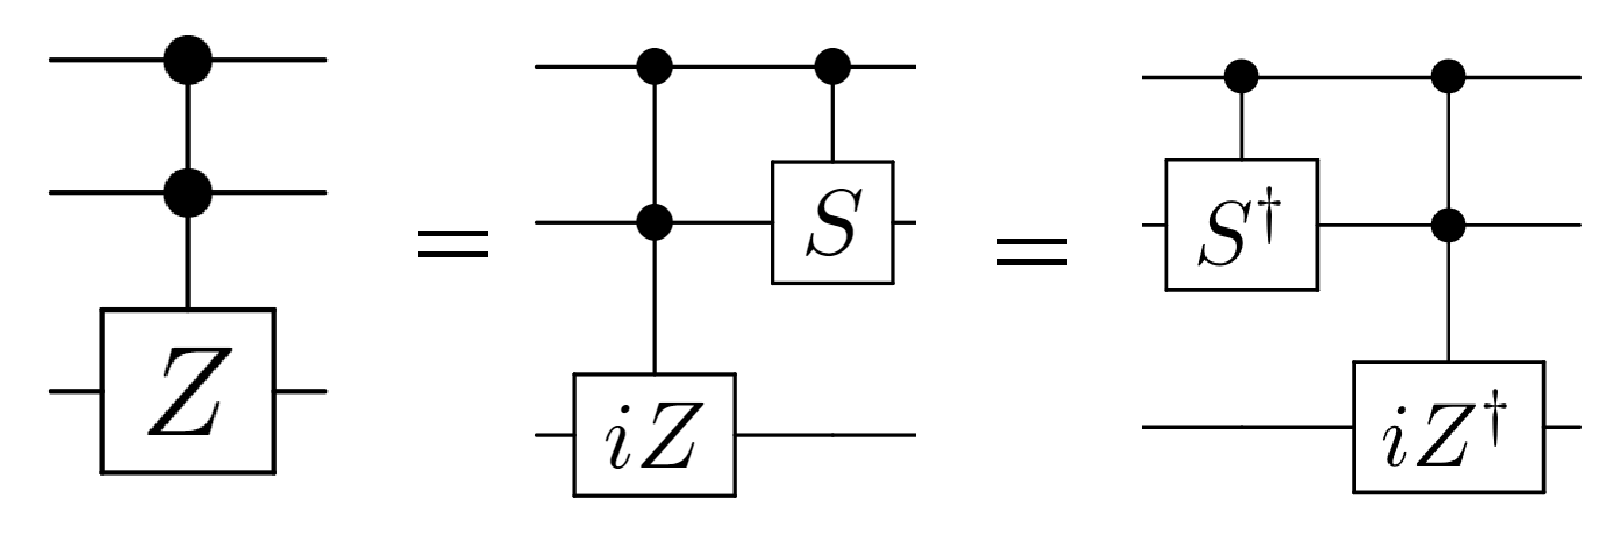
\includegraphics[width=0.5\columnwidth]{img/zgate_to_izgate.pdf}
  \caption{$CCZ$ゲートから$CCiZ, CS$ゲート,$CCiZ^{\dag}, CS^{\dag}$ゲートへの置換}
  \label{zgate_to_iz}    
\end{figure}
\begin{figure}[tbp]
    \centering
    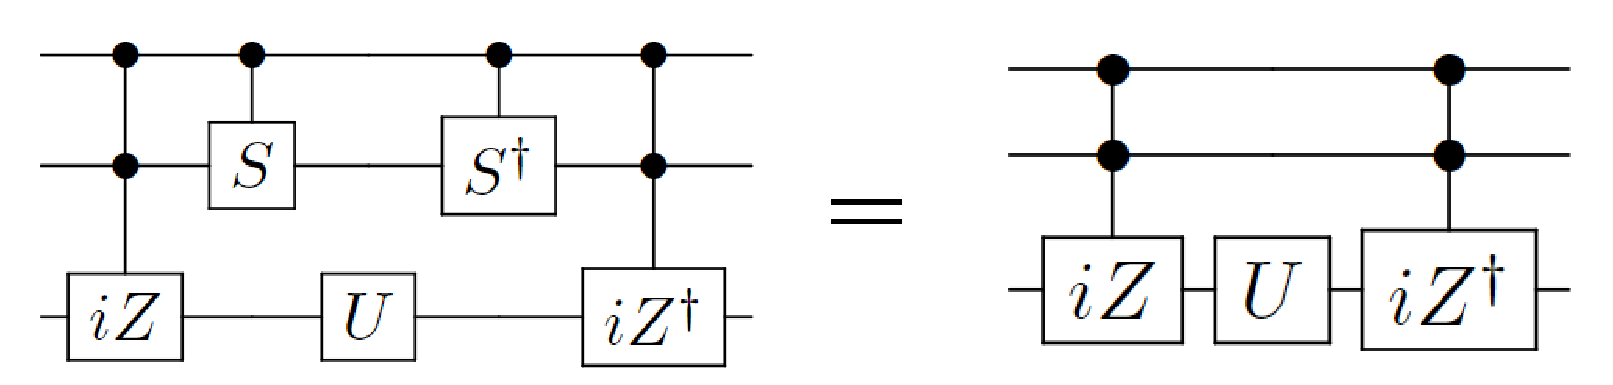
\includegraphics[width=0.5\columnwidth]{img/izgate_transformation.pdf}
    \caption{$CS, CS^{\dag}$ゲートの打ち消しあい}
    \label{izgate_transform}    
\end{figure}
\begin{figure}[tbp]
  \centering
  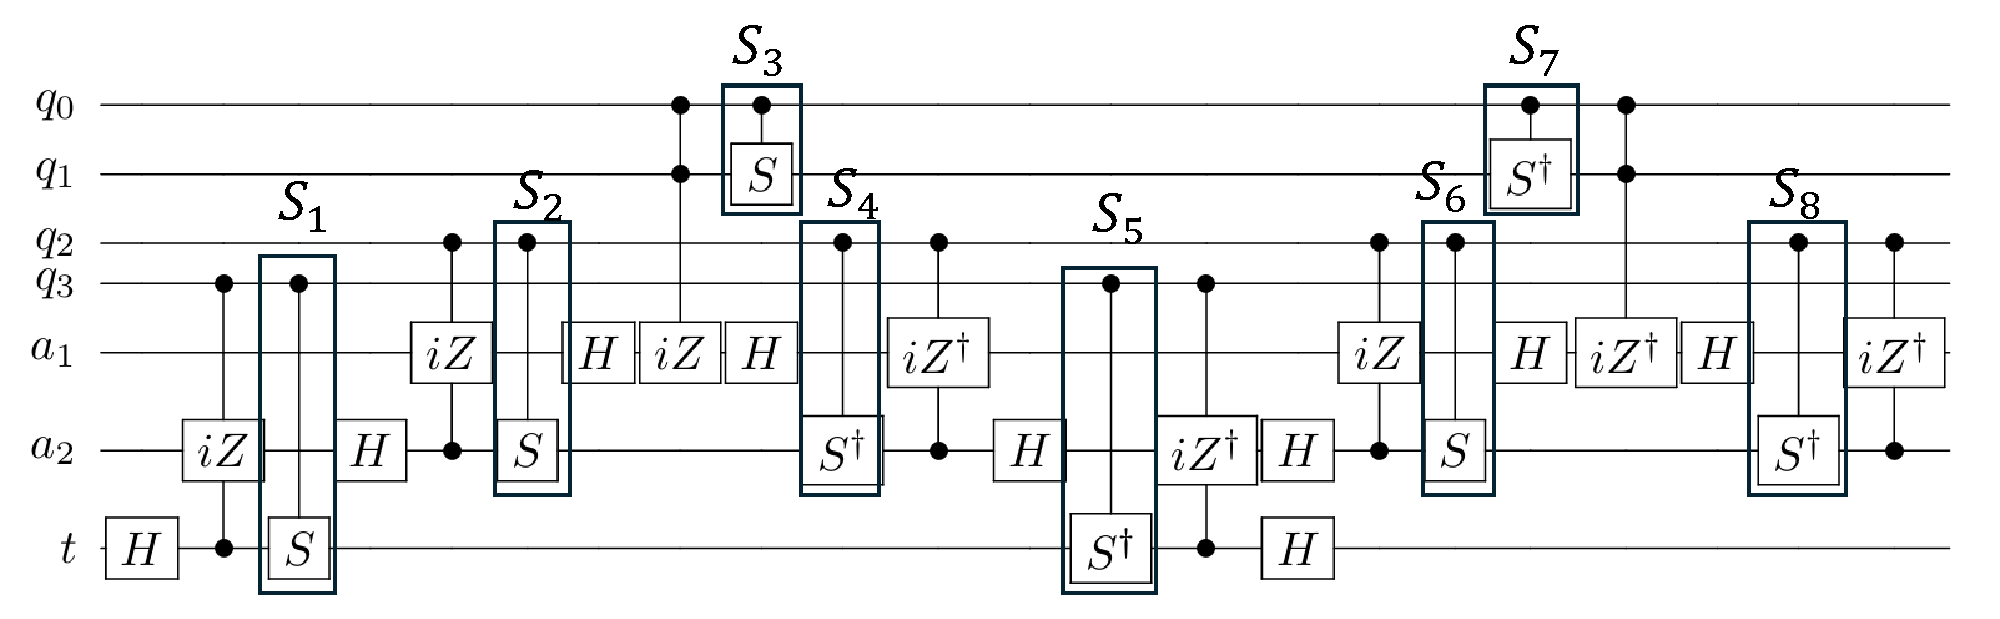
\includegraphics[width=14cm]{img/ccz_to_iz_cs.pdf}
  \caption{図~\ref{toffoli_to_ccz}の$CCZ$ゲートを$CCiZ, CS$ゲートと$CCiZ^{\dag}, CS^{\dag}$ゲートに置換した例}
  \label{ccz_to_iz_cs}
\end{figure}
\par
\mout{最後に,$CCiZ$ゲートを$CCi\omega Z$ゲートに置換する方法を説明する.
図~\ref{iz_to_iomegaz}に示すように,$CCiZ$ゲートは$CCi\omega Z$ゲートと$T^{\dag}$ゲートに置換でき,
$CCiZ^{\dag}$ゲートは$CCi\omega Z^{\dag}$ゲートと$T$ゲートに置換できる.
図~\ref{barenco_iz_to_iomegaz}に,図~\ref{ccz_to_iz_cs}の
$CCiZ, CCiZ^{\dag}$ゲートをそれぞれ,$CCi\omega Z, T^{\dag}$ゲートと$CCi\omega Z^{\dag}, T$ゲートに置換した例を示す.
図~\ref{barenco_iz_to_iomegaz}中の$T_{2}$と$T_{3}$は,それぞれの操作を打ち消しあっているため,
これらの$T, T^{\dag}$ゲートは削除できる.
図~\ref{barenco_iz_to_iomegaz}中の$T_{4}$は$T_{1}$の操作を復元する.
これらのゲートは,存在しなくても演算の結果に影響を与えることはないため,削除できる.
このように,演算に影響がない$T, T^{\dag}$ゲートを削除し,
$CCiZ$ゲートを$CCi\omega Z$ゲートに置換する.
結果として,
図~\ref{techmap}に示すように,
図~\ref{barenco}中で最も下側に位置するゲート$g_{1}, g_{5}$と,最も上側に位置するゲート$g_{3}, g_{7}$は$CCiZ, CCiZ^{\dag}$ゲートに置換できる.
また,図~\ref{barenco}中のゲート$g_{2}, g_{4}$と$g_{6}, g_{8}$は,それぞれ$CCi\omega Z, CCi\omega Z^{\dag}$ゲートに置換できる.}
\begin{figure}[tbp]
  \centering
  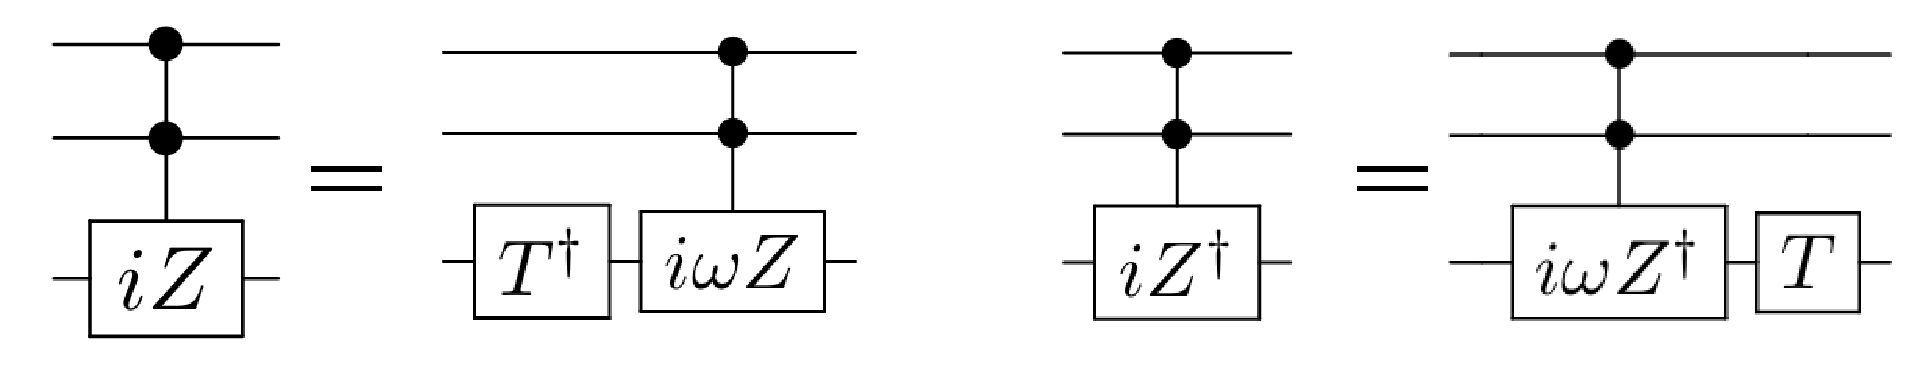
\includegraphics[width=11cm]{img/iz_to_iomegaz.pdf}
  \caption{\bout{$CCiZ$ゲートの$CCi\omega Z, T^{\dag}$ゲートへの置換と,$CCiZ^{\dag}$ゲートの$CCi\omega Z^{\dag}, T$ゲートへの置換}}
  \label{iz_to_iomegaz}
\end{figure}
\begin{figure}[tbp]
  \centering
  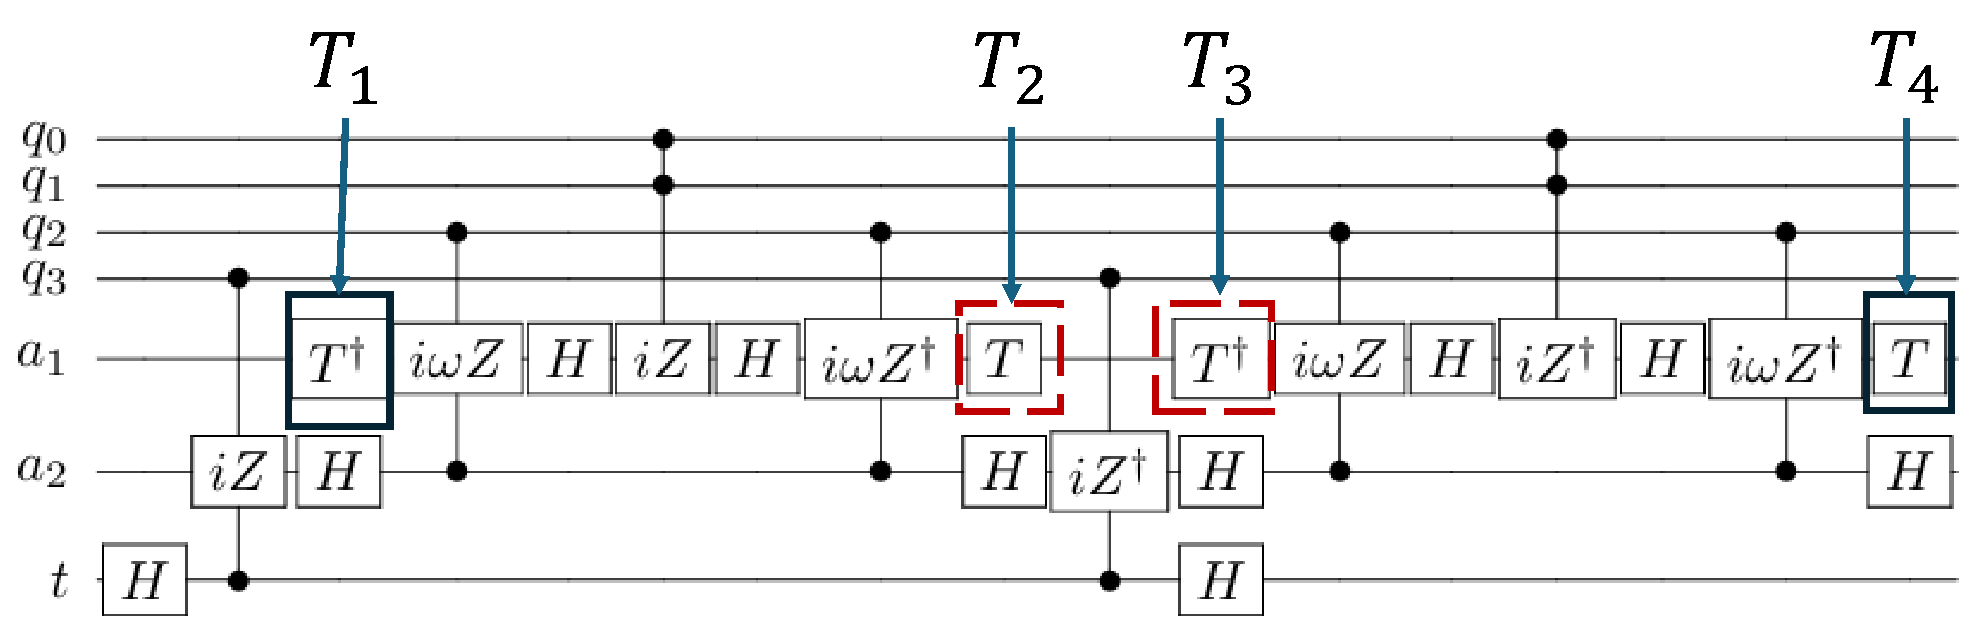
\includegraphics[width=14cm]{img/barenco_iz_to_iomegaz.pdf}
  \caption{図~\ref{ccz_to_iz_cs}の$CCiZ, CCiZ^{\dag}$ゲートをそれぞれ,$CCi\omega Z, T^{\dag}$ゲートと$CCi\omega Z^{\dag}, T$ゲートに置換した例}
  \label{barenco_iz_to_iomegaz}
\end{figure}
\begin{figure}[tbp]
  \centering
  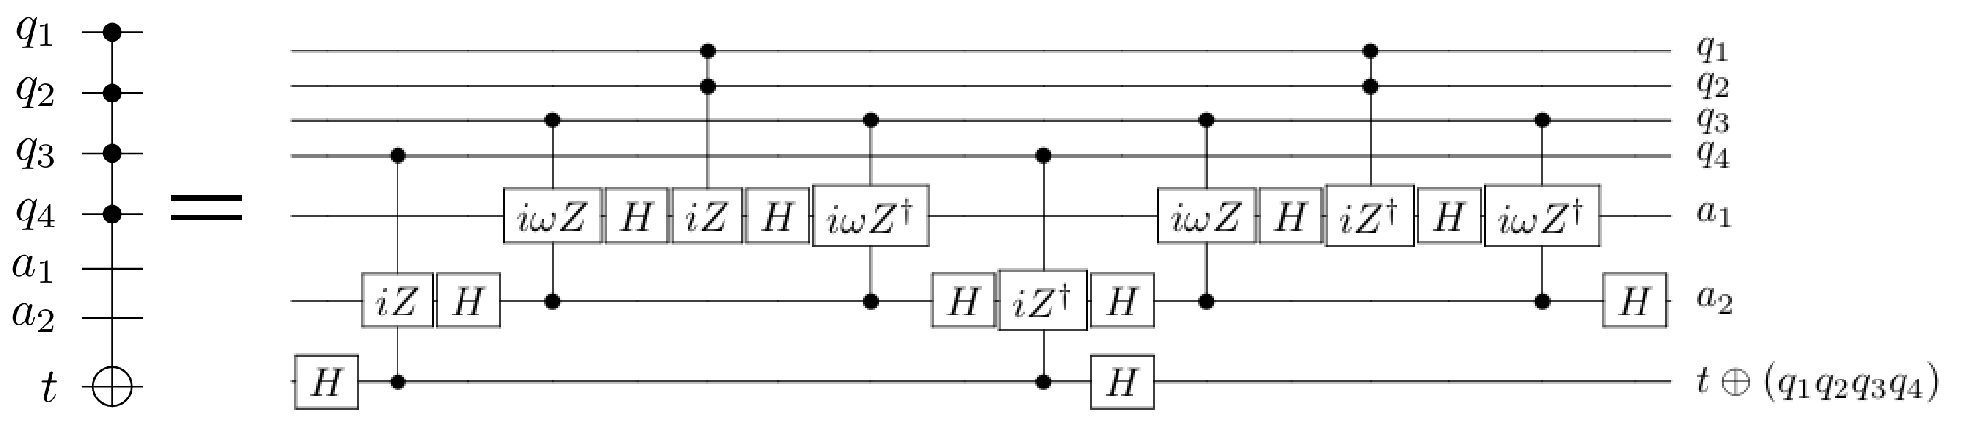
\includegraphics[width=0.9\columnwidth]{img/techmap.pdf}
  \caption{$c=4$のMCTゲートへの手法~1の適用例}
  \label{techmap}
\end{figure}
\par
手法~1は,MCTゲートを$c-2$個の補助ビットを用いて,
% 分解の説明をする普通に全部説明したほうが楽かも
4個の$CCiZ$ゲートと,$4(c-3)$個の$CCi\omega Z$ゲートに分解する.
$CCiZ$ゲートと,$CCi\omega Z$ゲートのClifford+Tへの分解をそれぞれ図~\ref{cciz},図~\ref{cciomegaz}に示す.
$CCiZ$ゲートのT-depthは2,$CCi\omega Z$ゲートのT-depthは1である.
そのため,手法~1で分解したMCTゲートの最大のT-depthは,$4(c-1)$である.
\begin{figure}[tbp]
  \centering
  \begin{minipage}[b]{0.49\columnwidth}
    \centering
    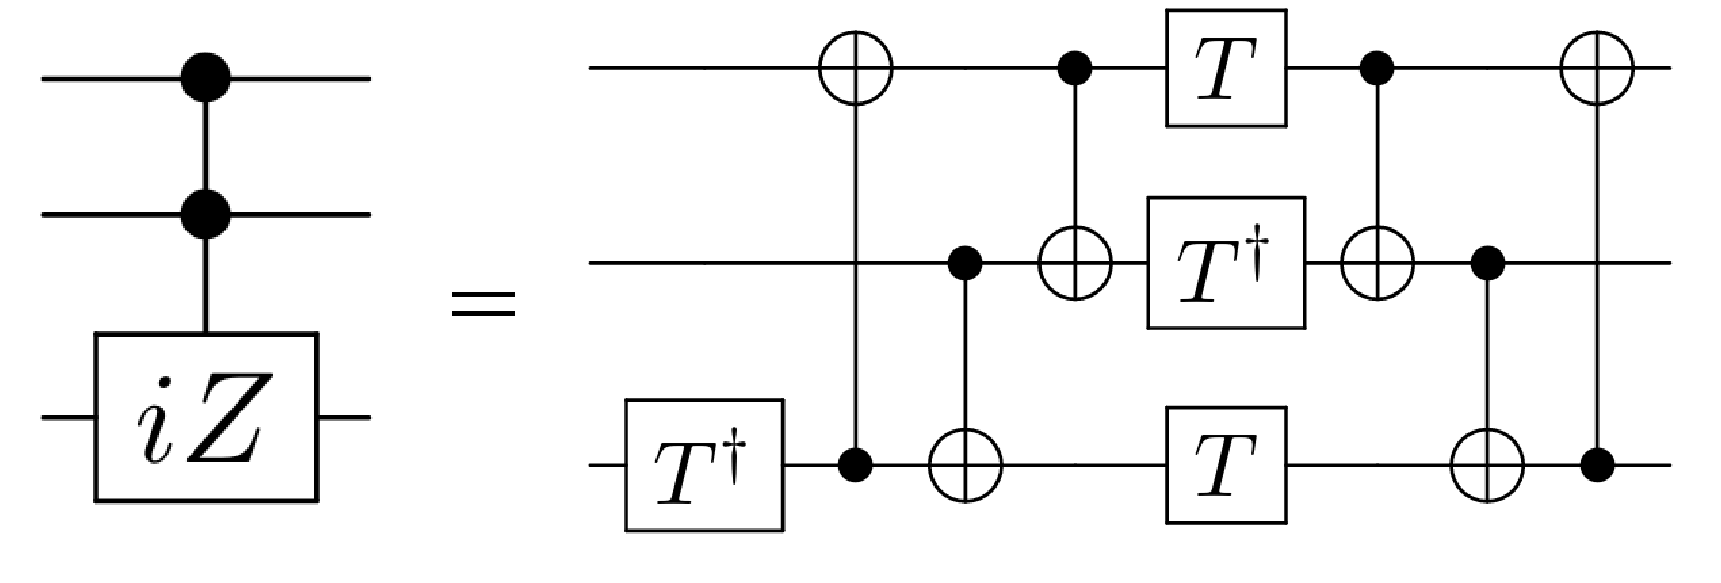
\includegraphics[width=0.9\columnwidth]{img/cciz.pdf}
    \caption{$CCiZ$ゲートのClifford+Tへの分解}
    \label{cciz}    
  \end{minipage}
  \begin{minipage}[b]{0.49\columnwidth}
    \centering
    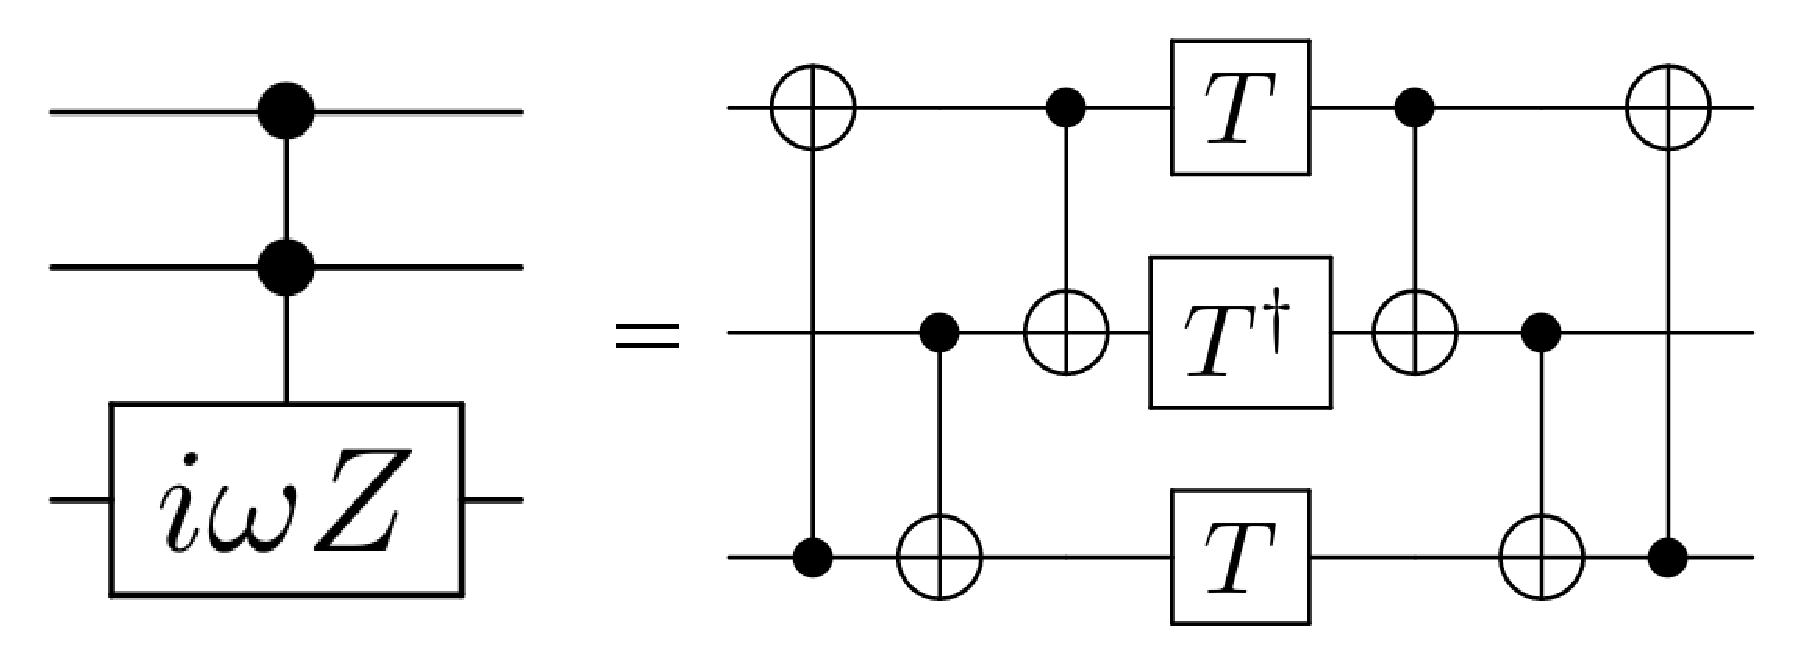
\includegraphics[width=0.9\columnwidth]{img/cciomegaz.pdf}
    \caption{$CCi\omega Z$ゲートのClifford+Tへの分解}
    \label{cciomegaz}    
  \end{minipage}
\end{figure}
\section{手法~2}
本節では,1個の値が不定の補助ビットを使用する分解手法\cite{abdessaied2016technology}について説明する.
以降,本手法を手法~2と呼ぶ.
\par
値が不定の補助ビットが\bout{$c-2$個未満のとき},MCTゲートを手法~1で分解することができない.
%コントロールビットを二つに分解することを説明する.
\bout{そこで,$c$個のコントロールビットを2つのビットの集合に分割する.
このとき,2つのビットの集合の要素数の差が1個以内となるよう分割する.}
そして,図~\ref{mimap}に示すように,
分割したビットの集合をコントロールビットに持つ4つのMCTゲート
$g_{1}, g_{2}, g_{3}, g_{4}$と4つの$C\omega S$ゲートにMCTゲートを一度分解する.
\begin{figure}[tbp]
  \centering
  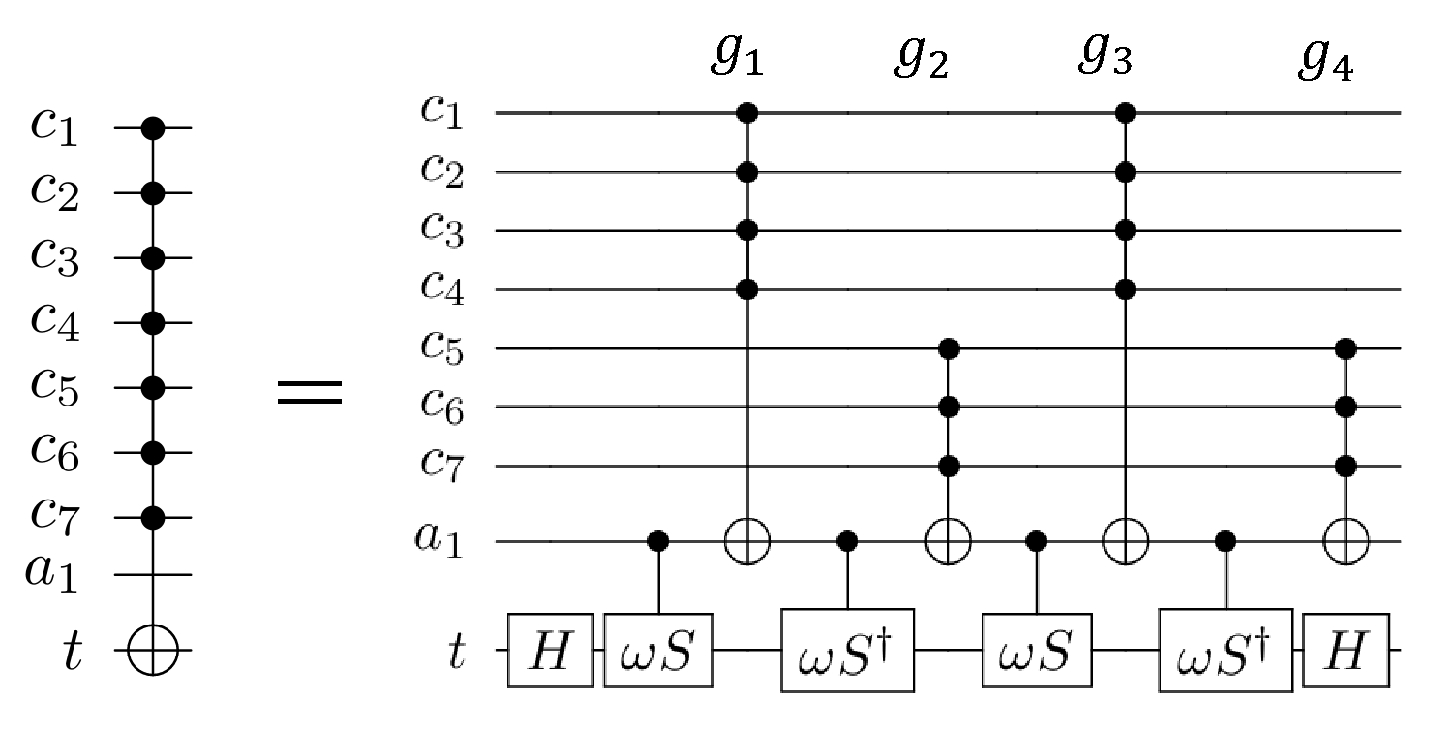
\includegraphics[width=11cm]{img/mimapping.pdf}
  \caption{$c=7$のMCTゲートへの手法~2の適用例}
  \label{mimap}
\end{figure}
ここで,$g_{3}$は$g_{1}$の,$g_{4}$は$g_{2}$の複製である.
\begin{figure}[tbp]
  \centering
  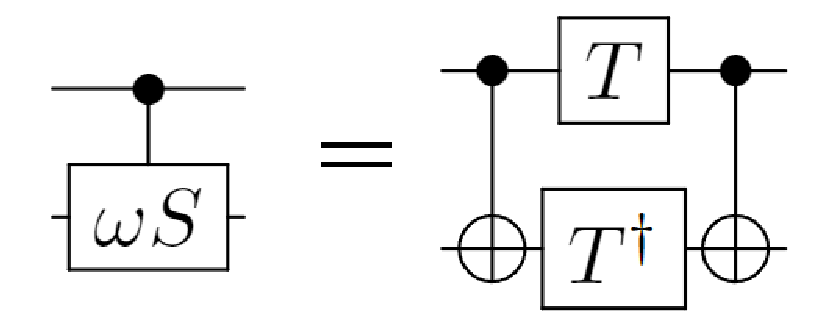
\includegraphics[width=5cm]{img/comegas.pdf}
  \caption{$C\omega S$ゲートのClifford+Tへの分解}
  \label{comegas}
\end{figure}
図~\ref{comegas}に示すように,
$C\omega S$ゲートは,補助ビットを用いずに,直接Clifford+Tへ分解できるゲートである.
手法~2では,
この分解した4つのMCTゲートに対し,手法~1を適用することで,MCTゲートをClifford+Tへ分解することができる.
\par
手法~2では,図~\ref{mimap}の$g_{3}$を$g_{1}$の分解に対し,$g_{4}$を$g_{2}$の分解に対し,
同じ補助ビットを使い,逆変換のゲートに置換したうえで,逆順に分解することで,T-depthを削減する.
\mout{
図~\ref{mimap_g2_g4}に
図~\ref{mimap}中の$g_{2}$を分解し,
$g_{4}$を$g_{2}$の分解に対し,逆変換のゲートに置換し,逆順に分解した例を示す.
図~\ref{mimap_g2_g4}の$G_{2}, G_{4}$は,$g_{2}, g_{4}$の分解を表す.
$G_{4}$は$G_{2}$を構成するゲートを逆変換のゲートに置換し,逆順にしたものである.}
\begin{figure}[tbp]
  \centering
  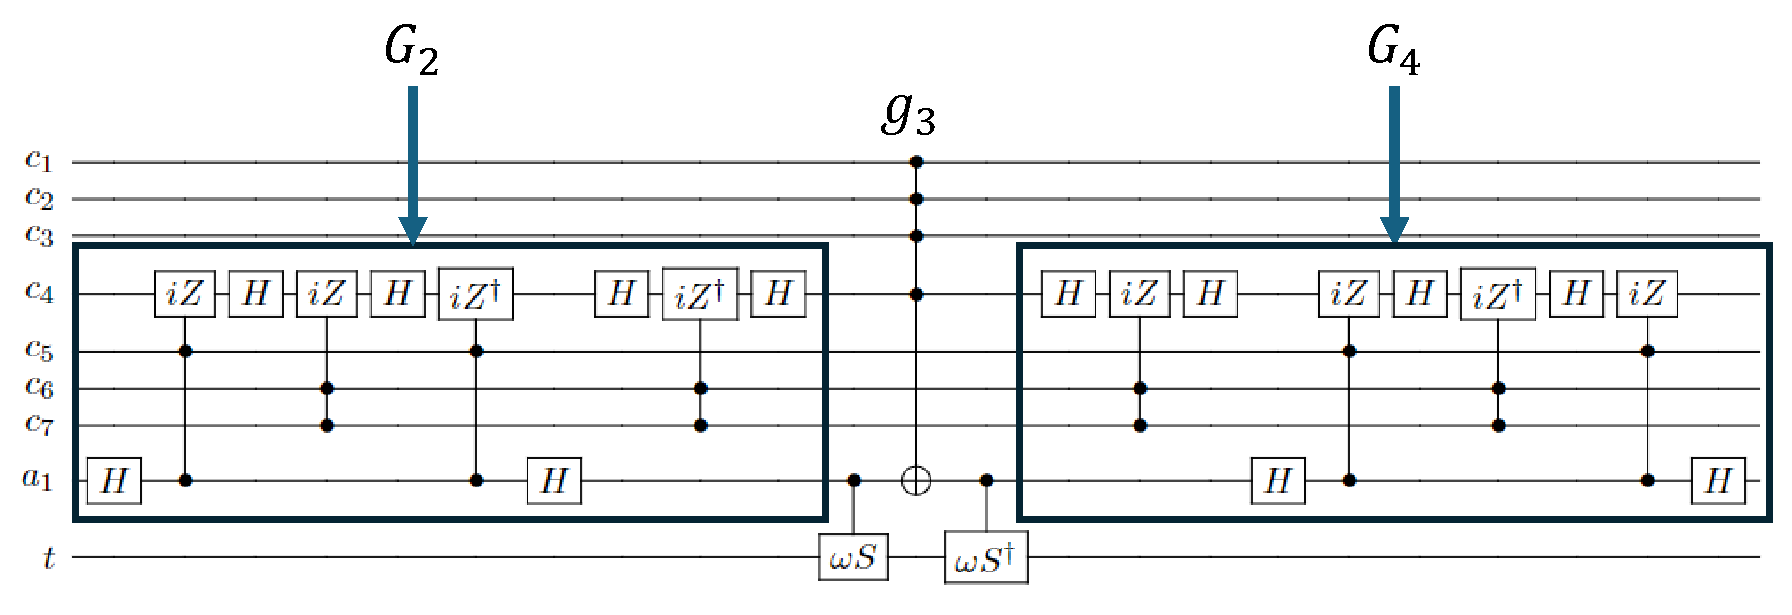
\includegraphics[width=15cm]{img/mimap_g2_g4.pdf}
  \caption{\mout{図~\ref{mimap}の$g_{2}$を分解し,$g_{4}$を$g_{2}$の分解に対し逆変換のゲートに置換し,逆順に分解した例}}
  \label{mimap_g2_g4}
\end{figure}
図~\ref{iz_to_iomegaz}に示すように,
\bout{$CCiZゲート$と$CCiZ^{\dag}$ゲートはそれぞれ,
$CCi\omega Z, T^{\dag}$ゲートと$CCi\omega Z^{\dag}, T$ゲートに置換できる.}
図~\ref{mimap_g2_g4}の\bout{$CCiZゲート$と$CCiZ^{\dag}$ゲートをそれぞれ,
$CCi\omega Z, T^{\dag}$と$CCi\omega Z^{\dag}, T$ゲートに}
置換した例を図~\ref{mimap_g2_g4_trans}に示す.
\mout{
図~\ref{mimap_g2_g4_trans}の$T$ゲート$T_{4}$は,
$T^{\dag}$ゲート$T_{1}$の操作を復元する.
これらのゲートは,存在しなくても演算の結果に影響を与えることはないため,削除できる.
同様に図~\ref{mimap_g2_g4_trans}の$T_{2}, T_{3}$についても削除できる}.
\par
このようにして,$g_{1}, g_{3}$の組と$g_{2}, g_{4}$の組を分解することで,
合計8つの$CCiZ, CCiZ^{\dag}$ゲートを$CCi\omega Z, CCi\omega Z^{\dag}$ゲートへ置換でき,\mout{置換を行う前からT-depthを8削減できる.
コントロールビットの差を一つ許容して均等に分割するため,
置換を行う前の4つのMCTゲートを手法1で分解した合計のT-depthは,
$2 \cdot  4(\lfloor \frac{c}{2}  \rfloor -1) +2\cdot 4(\lceil \frac{c}{2} \rceil -1)=8(c-1)$となる.
また,4つの$C\omega S$ゲートを使用しているため,これらのゲートの合計のT-depthは$4$である.}
このため,手法~2を用いてコントロールビット数が$c$個のMCTゲートを
分解したときの最大のT-depthは$8(c-1)-8+4=8c-20$となる.
\begin{figure}[tbp]
  \centering
  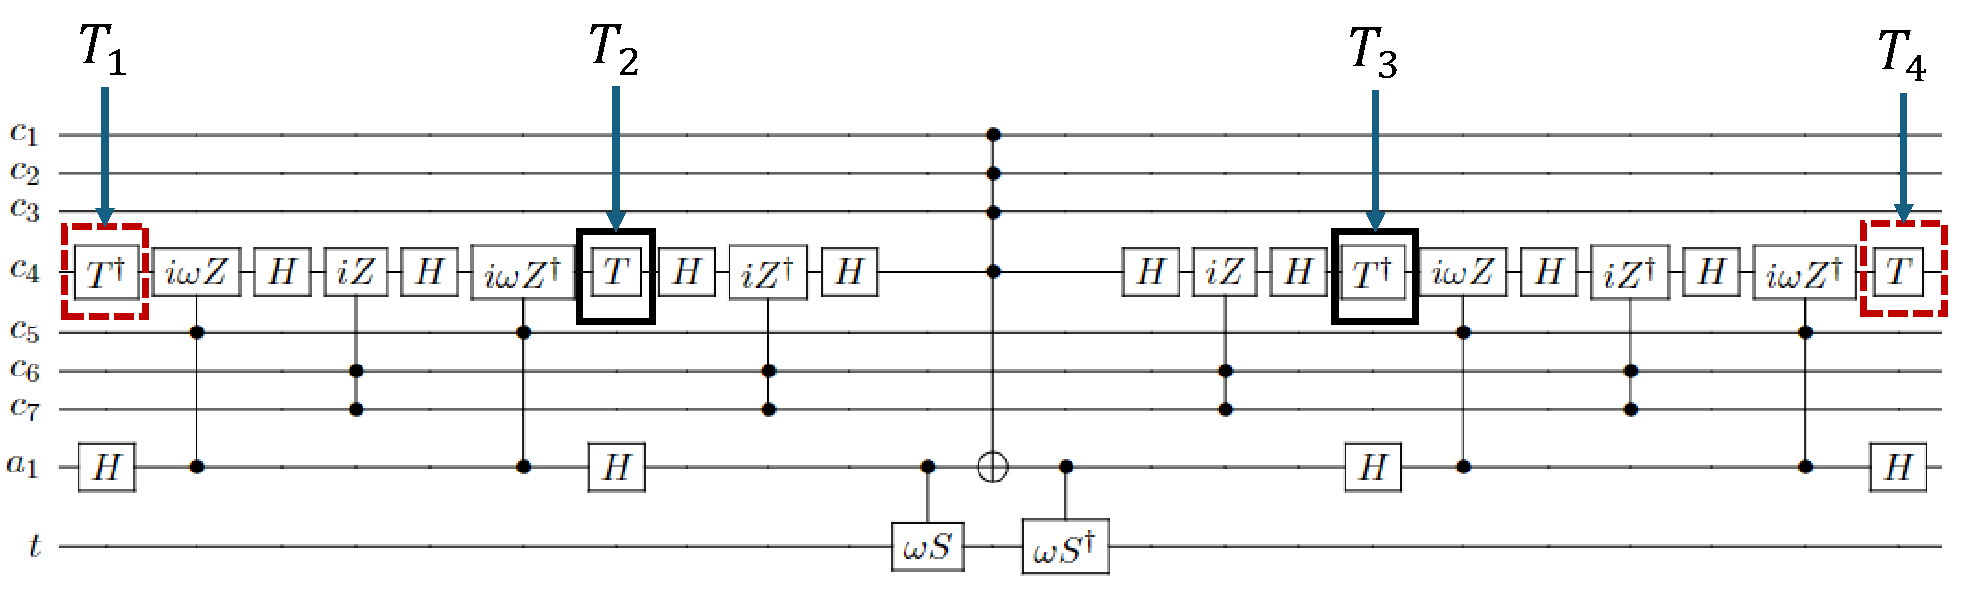
\includegraphics[width=18cm]{img/mimap_g2_g4_transform.pdf}
  \caption{図~\ref{mimap_g2_g4}の\bout{$CCiZ, CCiZ^{\dag}$ゲートをそれぞれ,$CCi\omega Z, T^{\dag}$ゲートと$CCi\omega Z^{\dag}, T$ゲートへ置換した例}}
  \label{mimap_g2_g4_trans}
\end{figure}
\section{手法~3}
本節では,2から$c-3$個の値が不定の補助ビットを使用し,MCTゲートを分解する手法\cite{baker2019decomposing}について説明する.
以降,本手法を手法~3と呼ぶ.
図~\ref{baker}に示すように,
\mout{\rout{必要な複製の数}が少ないMCTゲート$g_{1}$または$g_{4}$に,
多くのコントロールビットを使用し,分解することで,T-depthを削減する手法が手法~3である.
図~\ref{baker}の$g_{1}$の複製は$g_{7}$のみであるが,
$g_{2}$の複製は,$g_{6}, g_{8}, g_{13}$であるため,
$g_{1}$はその複製の数が少ないゲートといえる.
$g_{4}$についても,複製は$g_{10}$のみである.}
\par
手法~3の分解方法について説明する.
分解するMCTゲートの$c$個のコントロールビットの集合を$C$とする.
分解するMCTゲートのターゲットビットを$t$とする.
\mout{MCTゲートの分解に使用できる,$m$個の値が不定の補助ビットを$a_{1}, a_{2}, \dots, a_{m}$とする.}
図~\ref{baker}のように,$g_{1}, g_{2}, g_{3}, g_{4}$の配置が決定すれば,
$g_{4}$より右側にあるゲートは,$g_{1}, g_{2}, g_{3}, g_{4}$の複製であるため手法~3の分解は\rout{決定}できる.
すなわち,左側から$m+1$個分のゲートを構成するビットの配置が決定すれば,手法~3の分解を\rout{決定}できる.
この左側から$m+1$個のMCTゲートをそれぞれ$g_{1},\dots,g_{m+1}$とする.
$g_{1},\dots ,g_{m+1}$の持つ,コントロールビットの集合をそれぞれ$C_{1}, C_{2}, \dots ,C_{m+1}$で表す.
また,集合の要素数は,$|C_{i}|$で表す.
ここで,次の手順に則り,コントロールビットの集合$C_{1},\dots ,C_{m+1}$を構成するビットを決定する.
\begin{enumerate}[手順1]
  \item $C_{1}, \dots ,C_{m}$に$a_{1},\dots,a_{m}$を一つずつ移動する.
  \item $C_{1},\dots, C_{m+1}$の要素数が全て2になるように,\mout{$C$から$C_{i}$に要素を移動する.}
  \item $C_{1}$が$|C_{1}|-2 \leq c+m-|C_{1}|$である限り,\mout{$C$から$C_{1}$に要素を移動する.}
  \item $|C|=0$でなければ,\mout{$C_{m+1}$に,$C$の残りの要素を移動する.}
\end{enumerate}
\par
次に,$g_{1},\dots ,g_{m+1}$のターゲットビットの決定方法について説明する.
$g_{1}$のターゲットビットは,分解前のMCTゲートのターゲットビット$t$である.
$g_{i\geq 2}$のターゲットビットは,手順1で分配した$C_{i-1}$\mout{に含まれるビットである.}
このようにして,$g_{1},\dots, g_{m+1}$のビットの配置を決定する.
\par
$g_{1},\dots ,g_{m+1}$の構成するビットが決定すれば,
回路の左側から式~\ref{eq:bakerhaiti}の順でゲートを配置する.
\begin{equation}\label{eq:bakerhaiti}
  \{g_{1}, g_{2}, \dots, g_{m+1}\},\{g_{m},g_{m-1}, \dots, g_{1}\}, \{g_{2}, g_{3} \dots, g_{m+1}\}, \{g_{m}, g_{m-1}, \dots, g_{2}\}
\end{equation}
配置したゲートのうちコントロールビットが3個以上のゲートに関しては,手法~1により分解する.
\begin{figure}[tbp]
  \centering
  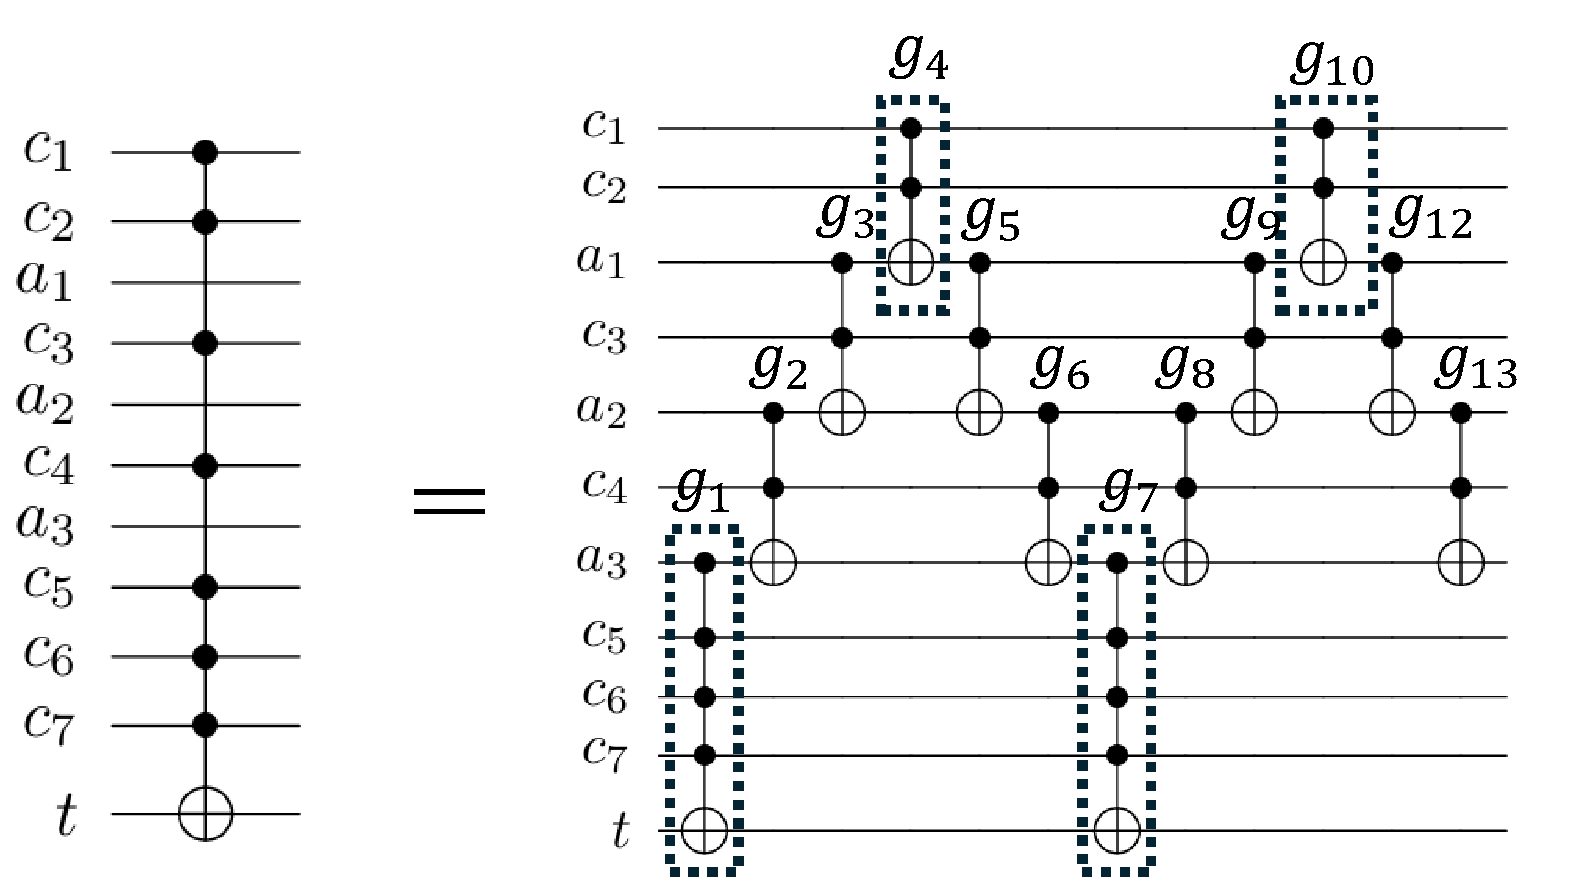
\includegraphics[width=10cm]{img/baker.pdf}
  \caption{値が不定の補助ビットが3個の時の$c=7$のMCTゲートへの手法~3の適用例}
  \label{baker}
\end{figure}
\par
MCTゲートに手法~3の分解を適用した際に現れるToffoliゲートは,$CCiZ, CCi\omega Z$ゲートに置換できる.
この方法について説明する.
まず,図~\ref{baker}上のToffoliゲートは,$CCiZ, CCiZ^{\dag}$ゲートに置換することができる.
図~\ref{baker_cciz}にその例を示す.
\begin{figure}[tbp]
  \centering
  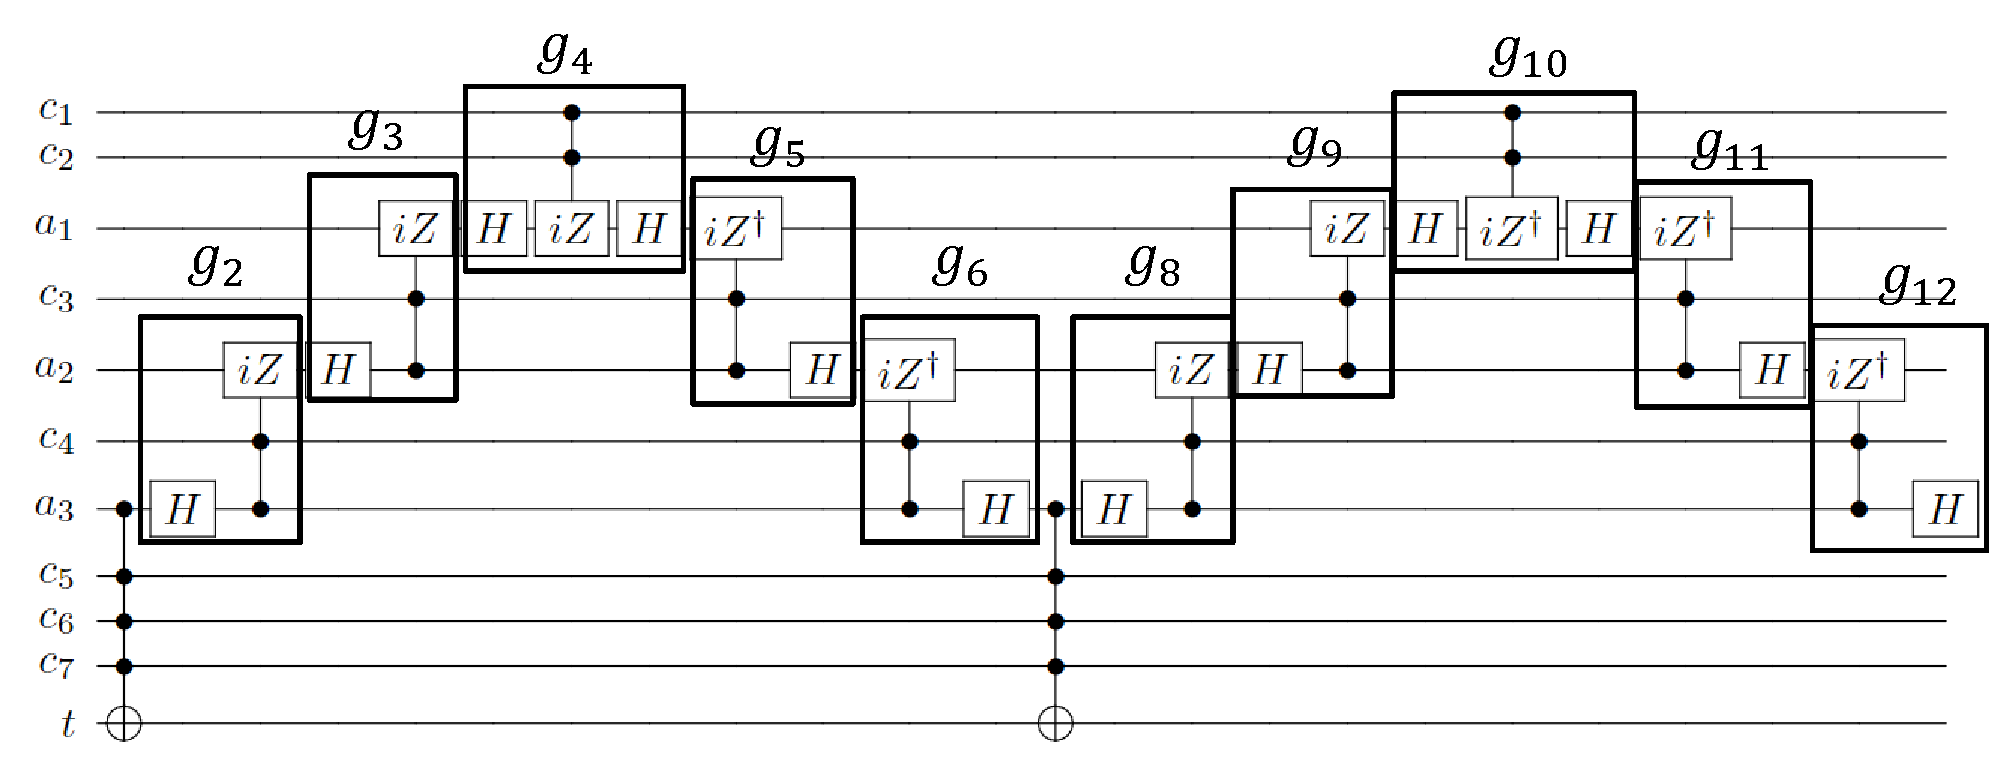
\includegraphics[width=15cm]{img/baker_izgate_transform.pdf}
  \caption{図~\ref{baker}のToffoliゲートの$CCiZ$ゲートへの置換}
  \label{baker_cciz}
\end{figure}
同じビットを入力と出力に持つToffoliゲートの組は,
図~\ref{toffoli_transform}のように$CCZ$ゲートに置換できる.
図~\ref{zgate_transform}に示すように,
$CCZ$ゲートは,ターゲットビットとコントロールビットを同一に見なすことができる.
図~\ref{zgate_to_iz}に示すように,$CCZ$ゲートは,$CCiZ$ゲートと$CS$ゲートか,$CCiZ^{\dag}$ゲートと$CS^{\dag}$ゲートに置換できる.
図~\ref{izgate_transform}に示すような配置の,$CS$ゲートと,$CS^{\dag}$ゲートは,互いの操作を打ち消しあう.
そのため,$CS$ゲートと,$CS^{\dag}$ゲートを消去しても同じ演算を表現できる.
このように,同じ入力と出力を持つToffoliゲートの組を,$CCiZ, CCiZ^{\dag}$ゲートの組に置換することができる.
そのため,図~\ref{baker}のToffoliゲートを図~\ref{baker_cciz}のように$CCiZ, CCiZ^{\dag}$ゲートに置換できる.
\par
図~\ref{baker_cciomegaz}に示すように,
図~\ref{baker_cciz}の
\bout{$CCiZ, CCiZ^{\dag}$ゲートはそれぞれ,$CCi\omega Z$ゲートと$T^{\dag}$ゲート, 
$CCi\omega Z^{\dag}$ゲートと$T$ゲートに置換できる.}
図~\ref{baker_cciomegaz}の
\mout{
$T, T^{\dag}$ゲート$T_{3}, T_{6}$と$T_{4}, T_{5}$は,互いの演算を打ち消し合うため,削除できる.
また,図~\ref{baker_cciomegaz}中の
$T^{\dag}, T$ゲート$T_{1}, T_{8}$と,$T_{2}, T_{7}$についても,
左側の$T_{1}, T_{2}$の\bout{$T^{\dag}$}ゲートの演算を右側の$T_{7}, T_{8}$の\bout{$T$ゲート}が復元している.}
これらのゲートが存在しなくても演算の結果に影響を与えることがないため,これらのゲートについても削除できる.
このようにして,手法~3の分解で現れるToffoliゲートは,$CCiZ, CCi\omega Z$ゲートに置換することができる.
\begin{figure}[tbp]
  \centering
  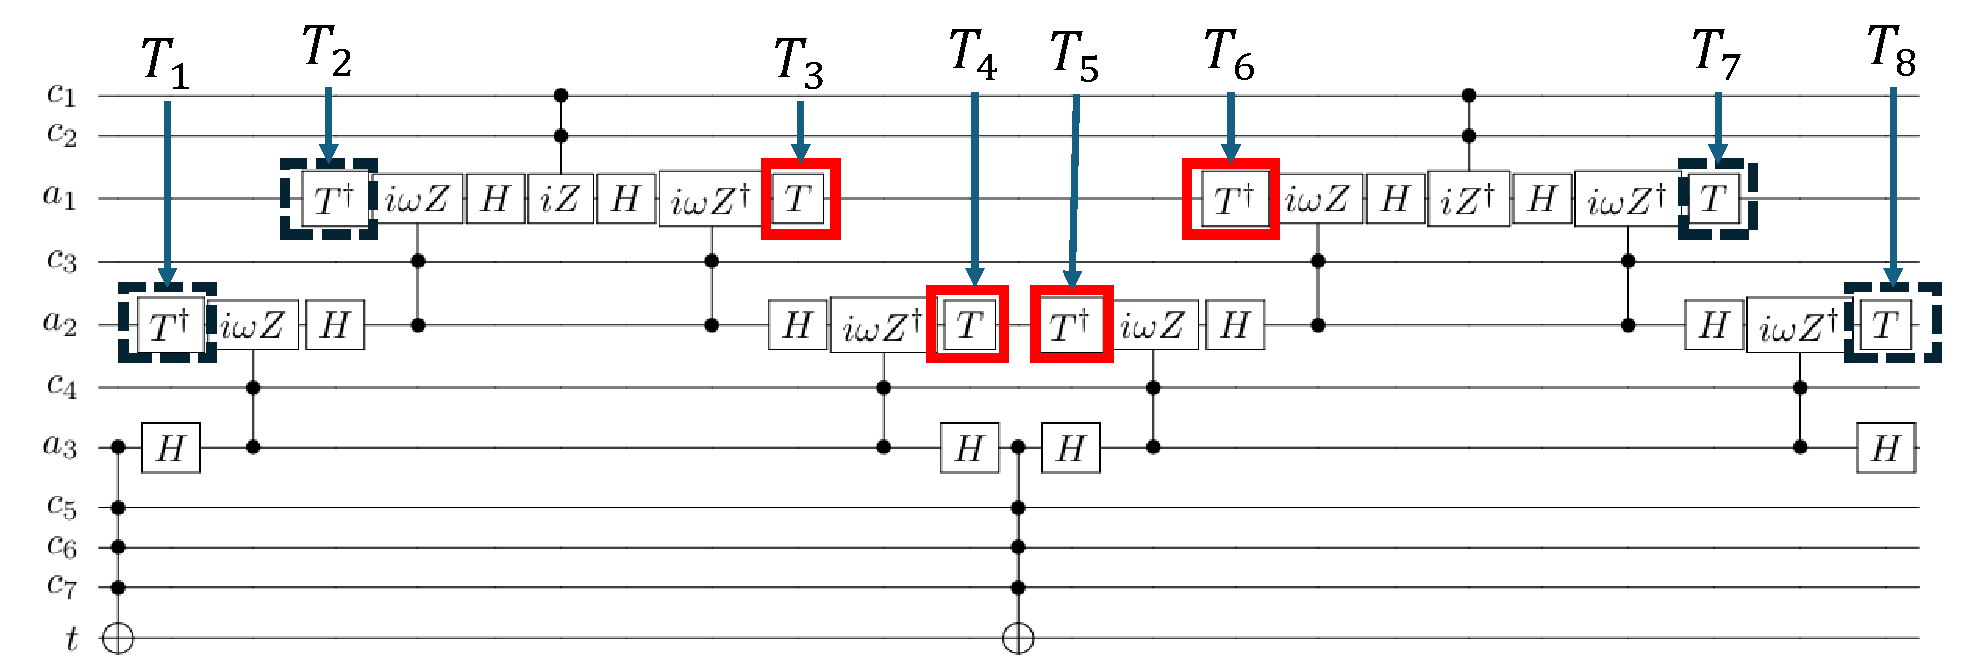
\includegraphics[width=15cm]{img/baker_iomegaz.pdf}
  \caption{図~\ref{baker_cciz}の\bout{$CCiZ, CCiZ^{\dag}$ゲートをそれぞれ,$CCi\omega Z, T^{\dag}$ゲートと$CCi\omega Z^{\dag}, T$ゲートに置換した例}}
  \label{baker_cciomegaz}
\end{figure}
\section{手法~4}
本節では,
値が0の補助ビットを用いたMCTゲートの分解手法\cite{niemann2019t}について説明する.
以降,本手法を手法~4と呼ぶ.
手法~4は,分解に使用する値が0の補助ビットの数$k$に\mout{よって場合分けして,}MCTゲートの分解を行う.
また,分解に使用する値が不定の補助ビット数を$d$とする.
$k$個の値が0の補助ビットを$a_{1},\dots, a_{k}$とする.分解を行うMCTゲートのコントロールビット数を$c$とする.
\subsection*{$1\leq k \leq \frac{c}{2}$の場合}
$1\leq k \leq \frac{c}{2}$の場合,
図~\ref{niemann}に示すように,分解するMCTゲートを3段のMCTゲートに分解する.
分解したMCTゲートそれぞれに,手法~1を適用し分解を行う.
手法~4では,図~\ref{niemann}のように,
$k$の数だけ1,3段目にMCTゲートを並列に配置することで,T-depthを削減する.
\par
MCTゲートを3段に分解する方法について説明する.
まず,分解するMCTゲートの$c$個のコントロールビットを
$k+1$個のコントロールビットの集合$C_{1},\dots,C_{k+1}$に分割する.
この分割したコントロールビットの集合の要素数は$|C_{i}|$と表す.
3段のMCTゲートの配置は次の通りである.
\begin{enumerate}[1段目]
  \item $C_{1},\dots, C_{k}$をそれぞれのコントロールビットとし,$a_{1},\dots,a_{k}$を
  それぞれのターゲットビットとする$k$個のMCTゲートを配置.
  \item $C_{k+1}$と$k$個の補助ビット$a_{1},\dots,a_{k}$をコントロールビットとし,
  ターゲットビットを元のMCTゲートのターゲットビット$t$とするMCTゲートを2段目に配置する.
  \item 3段目には1段目と同じ$k$個のMCTゲートを配置する.
  3段目のMCTゲートにより値が0の補助ビットの値を0に復元する.
\end{enumerate}
\begin{figure}[tbp]
  \centering
  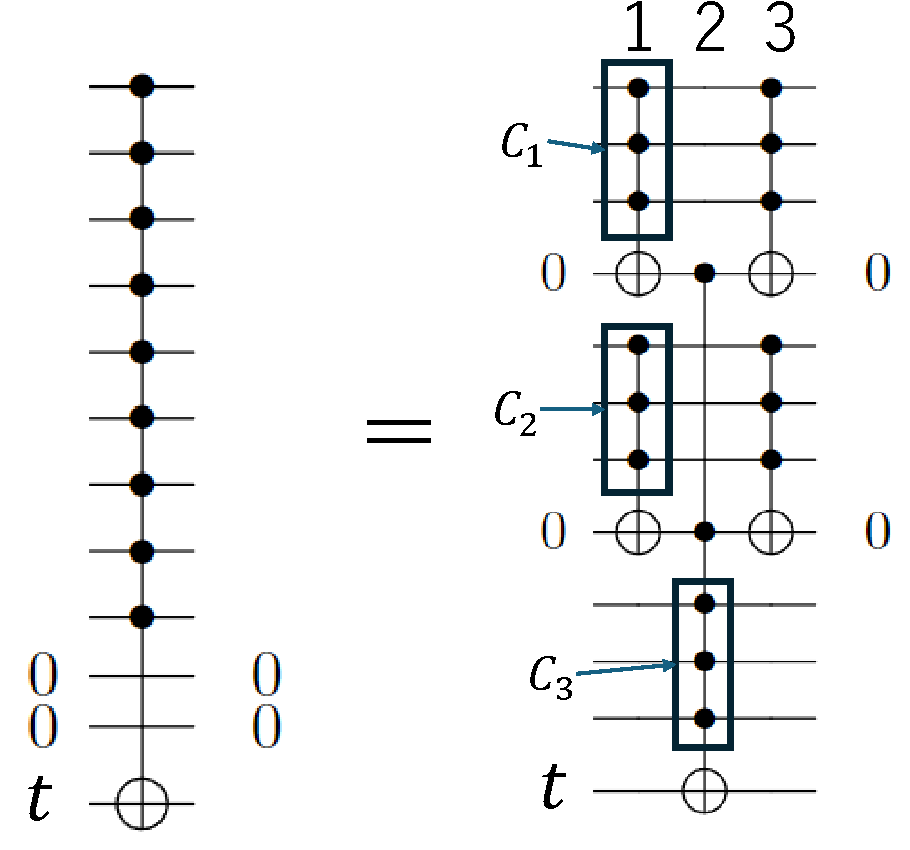
\includegraphics[width=6cm]{img/niemann.pdf}
  \caption{2つの値が0の補助ビットを用いた$c=9$のMCTゲートの分解例}
  \label{niemann}
\end{figure}
\par
3段に配置したMCTゲートの分解には,手法~1を用いる.
従って,これらのMCTゲートを分解するには,
それぞれのコントロールビットの数に応じた,値が不定の補助ビットが必要である.
各段に必要な値が不定の補助ビットの数を考慮して,
$C_{1},\dots,C_{k+1}$を決定する必要がある.
\par
2段目のMCTゲートは$k+|C_{k+1}|$個のコントロールビットを持つ.
そのため,2段目のMCTゲートに手法~1を適用するには,
$k+|C_{k+1}-2|$個の値が不定の補助ビットが必要である.
2段目のMCTゲートで使用されていないビットは,値が不定の補助ビットとして使用できる.
そのため,1段目でコントロールビットとして使用されている,
$|C_{1}|+,\dots, +|C_{k}|$個のビットは,
2段目のMCTゲートで値が不定の補助ビットとして使用できる.
2段目のMCTゲートに手法~1の分解を適用するには,
式~\ref{eq:2danme}を満たす必要がある.
\begin{equation}\label{eq:2danme}
  d+|C_{1}|+\dots +|C_{k}|\geq (k+|C_{k+1}|)-2
\end{equation}
\par
1,3段目のMCTゲートに手法~1を適用するには,
$(|C_{1}|-2)+\dots+(|C_{k}|-2)$個の値が不定の補助ビットが必要である.
1,3段目で用いられていないビットは値が不定の補助ビットとして利用できる.
そのため,
2段目でコントロールビットとして用いられる$|C_{k+1}|$個のビットと
2段目のターゲットビット$t$が値が不定の補助ビットとして利用できる.
加えて,分解に使用する値が不定の補助ビットの数$d$を考慮すると,1,3段目のMCTゲートに対して手法~1を適用するには,
式\ref{eq:13danme}を満たさなければならない.
\begin{eqnarray}\label{eq:13danme}
  d+|C_{k+1}|+1&\geq& (|C_{1}|-2)+\dots+(|C_{k}|-2)=|C_{1}|+\dots+|C_{k}|-2k
\end{eqnarray}
\par
$C_{1}+\dots +C_{k+1}=c$であることと,
式~\ref{eq:2danme}と式~\ref{eq:13danme}から,
式~\ref{eq:seiyaku}を導ける.
\begin{equation}\label{eq:seiyaku}
  \frac{c+2-k+d}{2}\geq|C_{k+1}|\geq \frac{c-2k-d-1}{2}
\end{equation}
MCTゲートを分解する際
$C_{k+1}$の値を式~\ref{eq:seiyaku}を満たすようにすれば,
分解した各MCTゲートに手法~1を適用できる.
\par
単に,式~\ref{eq:seiyaku}を満たすようにMCTゲートを分解すると,
全体のT-depthが大きくなる場合がある.
そのため,全体の\bout{T-depthが小さくなる}ように,
$C_{1},\dots,C_{k+1}$を決定しなければならない.
その決定の方法は,下記の3ステップからなる.
\begin{enumerate}[ステップ(1)]
  \item $|C_{k+1}|$を式\ref{eq:seiyaku}を満たす最大の値とする.
  そして,残りの$c-|C_{k+1}|$個のコントロールビットを$C_{1},\dots,C_{k}$に均等に移動する.
  この際,$|C_{1}|,\dots,|C_{k}|$の差は1まで許容する.
  \item $C_{k+1}$から$C_{1},\dots,C_{k}$に
  $|C_{1}|,\dots,|C_{k}|$の最大数が増えないよう,コントロールビットを移動する.
  この際,$|C_{k+1}|$が式\ref{eq:seiyaku}を満たすように移動する.
  \item  
  もし$k\geq 2$かつ3個以上のコントロールビットを$C_{k+1}$から式\ref{eq:seiyaku}を満たすように移動できるなら,
  $C_{1},C_{2}$にコントロールビットを一つずつ移動し,ステップ(2)に戻る.
  そうでないなら終了する.
\end{enumerate}
以上の手順に基づいて$C_{1},\dots,C_{k+1}$を決定し,MCTゲートを3段に分解する.
\par
\mout{
$k=\frac{c}{2}$個の値が0の補助ビットを用いて分解すると,
図~\ref{niemann_frac_c_2}に示すように,1,3段目のすべてのMCTゲートの
コントロールビット数が2となる.
このとき,1,3段目は最適なコントロールビットの分割となっている.
そのため,より多くの値が0の補助ビットを加えても,
1,3段目のコントロールビットはこれ以上分割できない.}
\begin{figure}[tbp]
  \centering
  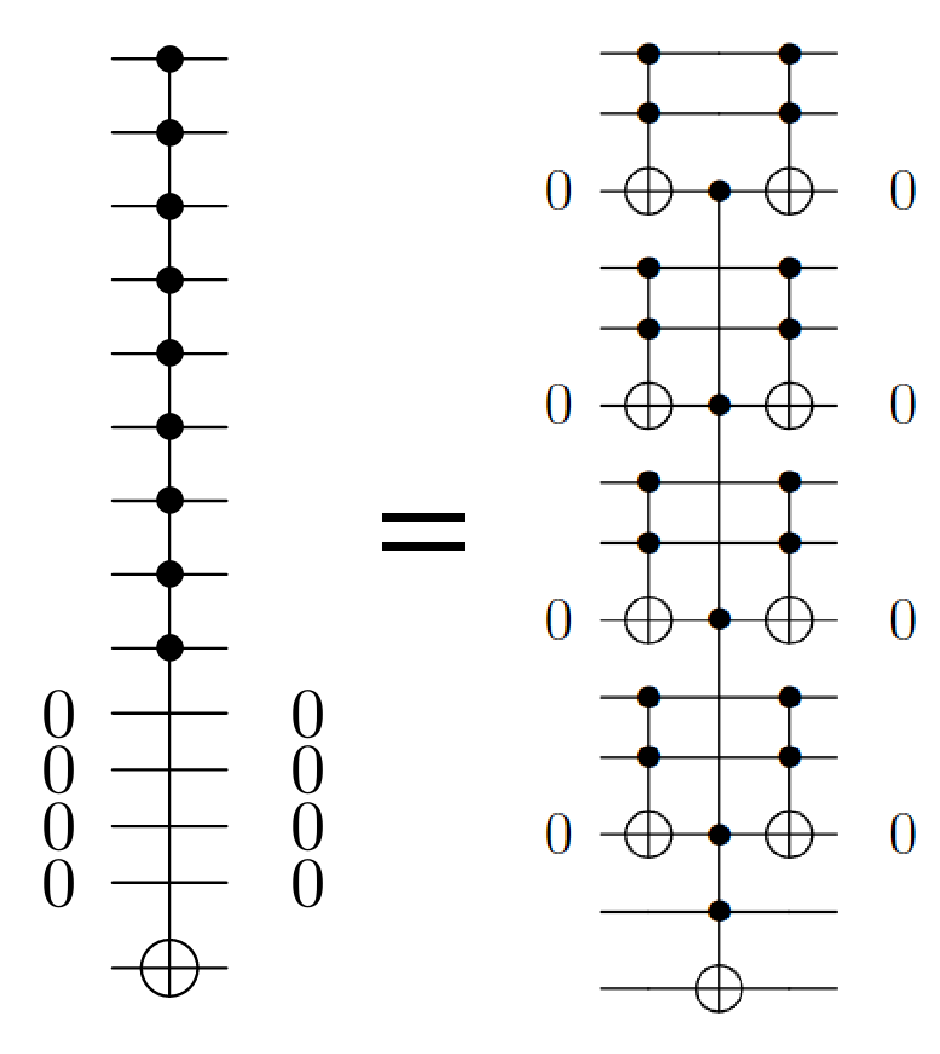
\includegraphics[width=8cm]{img/niemann_k_frac_c_2.pdf}
  \caption{4つの値が0の補助ビットを用いた$c=9$のMCTゲートの分解例}
  \label{niemann_frac_c_2}
\end{figure}
\subsection*{$\frac{c}{2} \bout{<} k \leq c-2$の場合}
\mout{$k>\frac{c}{2}$の場合では,
まず,$\lfloor\frac{c}{2}\rfloor$個の値が0の補助ビットを用いて,
1,3段目のすべてのMCTゲートをコントロールビット数が2となるよう分解する.
この際,2段目のMCTゲートのコントロールビットの数は,$c'=c-\lfloor \frac{c}{2}\rfloor$となる.
また,残りの値が0の補助ビット数は$k'=k-\lfloor \frac{c}{2} \rfloor$となる.
この残りの$k'$個の値が0の補助ビットを用いて,
\rout{$k'\leq \frac{c'}{2}$のときと,$k' > \frac{c'}{2}$の時に場合分けして,
2段目のコントロールビット数が$c'$のMCTゲートを分解する.}}
\par
\mout{
$k=c-2$のとき,
図~\ref{niemann_c_2}に示すように,
分解した全てのMCTゲートのコントロールビット数が2となる.
このため,$c-2$個より多くの値が0の補助ビットを加えても,
これ以上コントロールビットを分割できない.}
\begin{figure}[tbp]
  \centering
  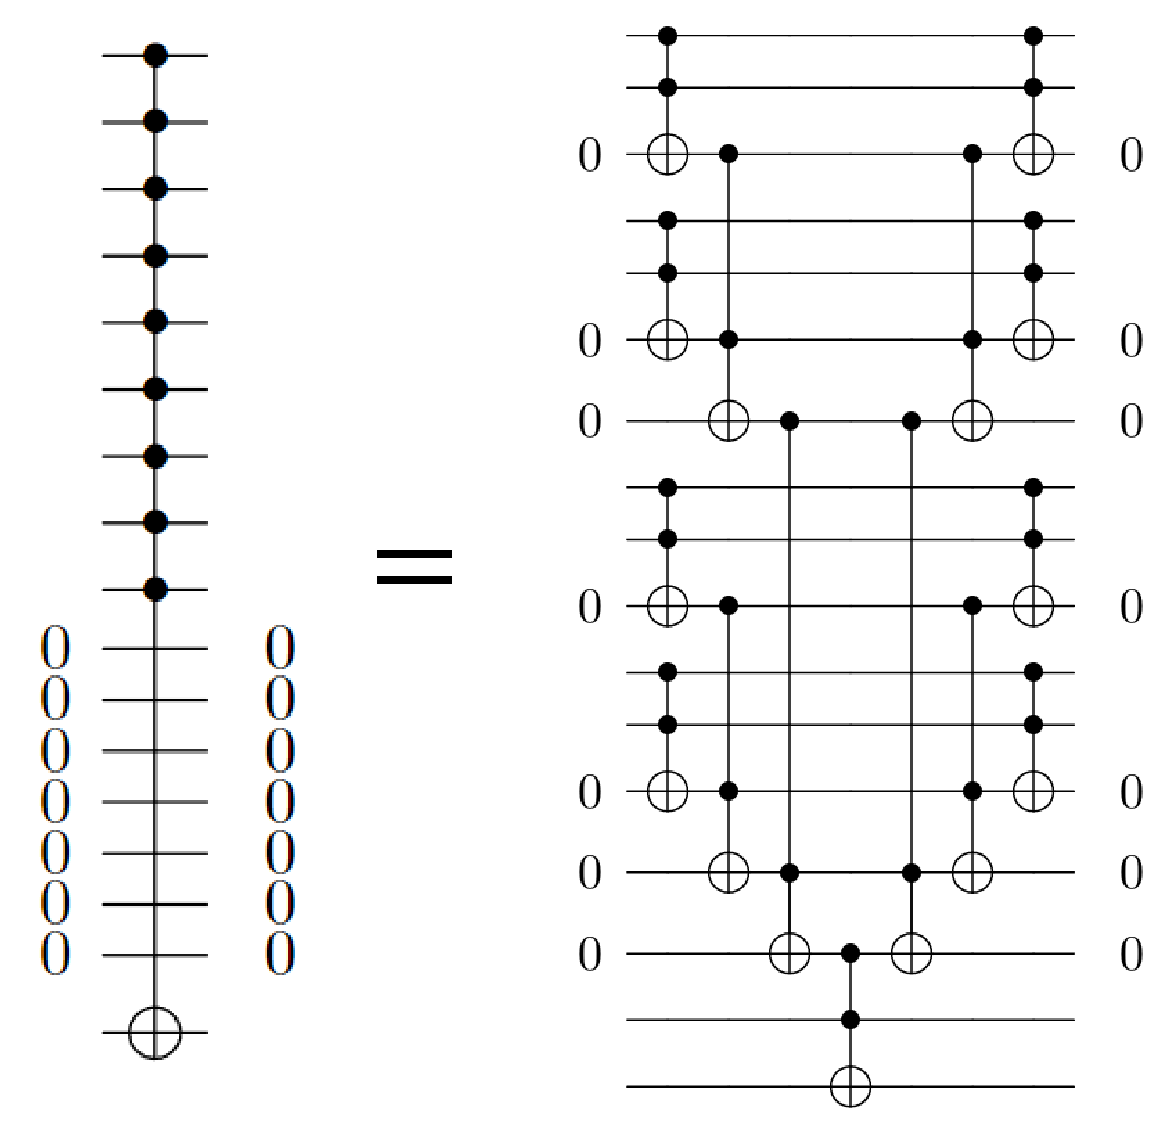
\includegraphics[width=9cm]{img/niemann_c_2.pdf}
  \caption{7つの値が0の補助ビットを用いた$c=9$のMCTゲートの分解例}
  \label{niemann_c_2}
\end{figure}